%%%%%%%%%%%%%%%%%%%%%%%%%%%%%%%%%%%%%%%%%
% Beamer Presentation
% LaTeX Template
% Version 1.0 (10/11/12)
%
% This template has been downloaded from:
% http://www.LaTeXTemplates.com
%
% License:
% CC BY-NC-SA 3.0 (http://creativecommons.org/licenses/by-nc-sa/3.0/)
%
%%%%%%%%%%%%%%%%%%%%%%%%%%%%%%%%%%%%%%%%%

%----------------------------------------------------------------------------------------
%   PACKAGES AND THEMES
%----------------------------------------------------------------------------------------

\documentclass{beamer}

\mode<presentation> {

% The Beamer class comes with a number of default slide themes
% which change the colors and layouts of slides. Below this is a list
% of all the themes, uncomment each in turn to see what they look like.

%\usepackage[utf8]{inputenc}
%\usefonttheme{professionalfonts} 
%\usefonttheme{serif}    
%\usepackage{tgbonum}
%\usepackage[T1]{fontenc}

%\usetheme{default}
%\usetheme{AnnArbor}
%\usetheme{Antibes}
%\usetheme{Bergen}
%\usetheme{Berkeley}
%\usetheme{Berlin}
%\usetheme{Boadilla}
%\usetheme{CambridgeUS}
%\usetheme{Copenhagen}
%\usetheme{Darmstadt}
%\usetheme{Dresden}
%\usetheme{Frankfurt}
%\usetheme{Goettingen}
%\usetheme{Hannover}
%\usetheme{Ilmenau}
%\usetheme{JuanLesPins}
%\usetheme{Luebeck}
\usetheme{Madrid}
%\usetheme{Malmoe}
%\usetheme{Marburg}
%\usetheme{Montpellier}
%\usetheme{PaloAlto}
%\usetheme{Pittsburgh}
%\usetheme{Rochester}
%\usetheme{Singapore}
%\usetheme{Szeged}
%\usetheme{Warsaw}

% As well as themes, the Beamer class has a number of color themes
% for any slide theme. Uncomment each of these in turn to see how it
% changes the colors of your current slide theme.

%\usecolortheme{albatross}
%\usecolortheme{beaver}
%\usecolortheme{beetle}
%\usecolortheme{crane}
%\usecolortheme{dolphin}
%\usecolortheme{dove}
%\usecolortheme{fly}
%\usecolortheme{lily}
%\usecolortheme{orchid}
%\usecolortheme{rose}
%\usecolortheme{seagull}
%\usecolortheme{seahorse}
%\usecolortheme{whale}
%\usecolortheme{wolverine}

%\setbeamertemplate{footline} % To remove the footer line in all slides uncomment this line
%\setbeamertemplate{footline}[page number] % To replace the footer line in all slides with a simple slide count uncomment this line
\usefonttheme[onlymath]{serif}
\setbeamertemplate{navigation symbols}{} % To remove the navigation symbols from the bottom of all slides uncomment this line
}
\usepackage{tikz}
\usetikzlibrary{calc}
\usepackage{graphicx} % Allows including images
\usepackage{booktabs} % Allows the use of \toprule, \midrule and \bottomrule in tables
\usepackage{svg}
\newcommand{\light}[1]{\textcolor{gray}{#1}}
%----------------------------------------------------------------------------------------
%   TITLE PAGE
%----------------------------------------------------------------------------------------

\title[L2Sum]{Learning 2 Summarize}
\author[Chris Kedzie]{Chris Kedzie, Columbia University\\
Fernando Diaz, Microsoft Research\\}

\institute[Columbia U.] % Your institution as it will appear on the bottom of every slide, may be shorthand to save space
{
%Computer Science Department \\
%Columbia University \\ % Your institution for the title page
\medskip
\textit{kedzie@cs.columbia.edu} % Your email address
}
\date{\today} % Date, can be changed to a custom date

\newcommand{\tikzmark}[1]{\tikz[overlay,remember picture] \node (#1) {};}

\usepackage{array}
\newcolumntype{L}[1]{>{\raggedright\let\newline\\\arraybackslash\hspace{0pt}}m{#1}}
\newcolumntype{R}[1]{>{\raggedleft\let\newline\\\arraybackslash\hspace{0pt}}m{#1}}


\begin{document}

\begin{frame}
\titlepage % Print the title page as the first slide
\end{frame}

%\begin{frame}
%\frametitle{Overview} % Table of contents slide, comment this block out to remove it
%\tableofcontents % Throughout your presentation, if you choose to use \section{} and \subsection{} commands, these will automatically be printed on this slide as an overview of your presentation
%\end{frame}

%----------------------------------------------------------------------------------------
%   PRESENTATION SLIDES
%----------------------------------------------------------------------------------------

\section{Motivation}
%\frame{\tableofcontents[currentsection]}
%\begin{frame}
%\frametitle{It's October 28th, 2012...}
%\vspace{10pt}
%\includegraphics<2>[scale=0.4]{png/news_anim1}
%\includegraphics<3>[scale=0.4]{png/news_anim2}
%\includegraphics<4>[scale=0.4]{png/news_anim3}
%\includegraphics<5>[scale=0.4]{png/news_anim4}
%\includegraphics<6>[scale=0.4]{png/news_anim5}
%\end{frame}
%





\begin{frame}
\frametitle{Last Year's Model: APSalience}

\begin{enumerate}
    \item Predict input sentence salience 
    \item Cluster input sentences (biased by step 1)
\end{enumerate}

\end{frame}

\begin{frame}
\frametitle{Last Year's Model: Salience Prediction}


Training data:

\begin{columns}[T] % align columns
\begin{column}{.48\textwidth}
Updates
\begin{itemize}
\item A packed train slammed into the end of the line in Buenos Aires' busy 
    Once station Wednesday, injuring over 300 morning commuters, 
    Argentina's transportation secretary said.
\item Earlier Wednesday, Schiavi said authorities believed there were problems with the train's brakes that caused it to smash into a barrier at the station.
\item[] \center $\vdots$
\end{itemize}
\end{column}%
\hfill%
\begin{column}{.48\textwidth}
Nuggets
\begin{itemize}
\item train accident in Buenos Aires, Argentina.
\item unknown number were killed
\item the train crashed at the buffer stop
\item the conductor seemed to struggle with the brakes
\item[] \center $\vdots$
\end{itemize}
\end{column}%
\end{columns}

\end{frame}

\begin{frame}
\frametitle{Last Year's Model: Salience Prediction}
    $\mathcal{N} = \{\textrm{train accident}, 
        \textrm{crashed at buffer}, \ldots, 
    \textrm{struggle with the brakes} \}$\\
    ~\\
    $s = \textrm{Schiavi said there were problems with the train's brakes} \ldots$\\
    \center
    $ \uncover<2>{\alert<2>{\operatorname{salience}(s)} =} \operatorname{max}_{n \in \mathcal{N}} \operatorname{sim}(n,s) = 
        \sum_i w_{i} \cdot \phi_{i}(s)  + b$ \\

\end{frame}

\begin{frame}
    \frametitle{Last Year's Model: Problems} 

    \begin{itemize}
        \item Salience model
            \begin{itemize}
                \item Difficult to incorporate dynamic features:
                    \begin{itemize}
                        \item stream observations
                        \item previous update similarity
                    \end{itemize}
            \end{itemize}
        \item[] ~\\
        \item Clustering
            \begin{itemize}
                \item Difficult to control over/under generating
                \item Increases latency penalties
                \item Limits scalability
            \end{itemize}
    \end{itemize}

\end{frame}


\begin{frame}
    \frametitle{This Year's Model}
\begin{columns}[T] % align columns
\begin{column}{.10\textwidth}
    ~\\~\\
    \def\svgwidth{\columnwidth}
    \only<1>{
        \resizebox{.35\textwidth}{!}{\input{seq1.pdf_tex}}
    }
    \only<2-3>{
        \resizebox{.35\textwidth}{!}{\input{seq2.pdf_tex}}
    }
    \only<4-5>{
        \resizebox{.35\textwidth}{!}{\input{seq3.pdf_tex}}
    }
    \only<6-7>{
        \resizebox{.35\textwidth}{!}{\input{seq4.pdf_tex}}
    }
\end{column}%
\hfill%
\begin{column}{.86\textwidth}
    ~\\
    ~\\
    \begin{tabular}{L{2.6cm} L{2.1cm} R{4.6cm}}
        $S=\{\}$ &    
        $U = \{\}$ & $ \uncover<2->{\textit{update}}\uncover<1>{?} = \operatorname{predict(s_1, U, S)}$\\
        ~\\
        \uncover<3->{$S=\{s_1\}$} &   
        \uncover<3->{$U = \{s_1\}$} & $ \uncover<4->{\textit{skip}}\uncover<3>{?}\uncover<3->{ = \operatorname{predict(s_2, U, S)}}$\\
        ~\\
        \uncover<5->{$S=\{s_1, s_2\}$} &  
        \uncover<5->{$U = \{s_1\}$} & 
        $ \uncover<6->{\textit{update}}\uncover<5>{?}\uncover<5->{ =  \operatorname{predict(s_3, U, S)}}$\\
        ~\\
        \uncover<7->{$S=\{s_1, s_2, s_3\}$} &  
        \uncover<7->{$U = \{s_1, s_3\}$} & $ 
        \uncover<7>{?} \uncover<7->{=  \operatorname{predict(s_4, U, S)}}$\\
    \end{tabular}
\end{column}%
\end{columns}

\end{frame}

\begin{frame}
     \[\operatorname{predict}(s, U, S)\]
        Feature representation:
        \begin{itemize}
            \item $\phi(s)$ --- language model scores, query scores, etc.
            \item<2-> $\alert<4>{\phi(s, U)}$ --- similarity to previous updates, etc.
            \item<3-> $\alert<4>{\phi(s, S)}$ --- number of documents in the stream, rolling 
                language models, etc.
        \end{itemize}
        \uncover<4>{\center Many features dependent on previous choices.}
\end{frame}

\begin{frame}
    \frametitle{Learning 2 Search --- Daume et. al. (2009)}

    structured prediction problem $\rightarrow$ search problem\\
~\\

    \begin{enumerate}
        \item the set of actions: $\mathcal{A} = \{update, skip \}$
        \item Each search state is:
            \begin{enumerate}
                \item observations from the stream $S=\{s_1, \ldots, s_{i-1}\}$
                \item a configuration of the update summary 
                        $U = \{s_a, s_b, s_c, \ldots\}$
                \item the current stream item $s_i$
            \end{enumerate}
    \end{enumerate}

\end{frame}

\begin{frame}
    \input{lols1.pdf_tex}
\end{frame}

\begin{frame}
    \input{lols2.pdf_tex}
\end{frame}
\begin{frame}
    \input{lols3.pdf_tex}
\end{frame}
\begin{frame}
    \input{lols4.pdf_tex}
\end{frame}
\begin{frame}
    \input{lols5.pdf_tex}
\end{frame}
\begin{frame}
    \input{lols6.pdf_tex}
\end{frame}
\begin{frame}
    \input{lols7.pdf_tex}
\end{frame}
\begin{frame}
    \input{lols8.pdf_tex}
\end{frame}
\begin{frame}
    \input{lols9.pdf_tex}
\end{frame}
\begin{frame}
    \input{lols10.pdf_tex}
\end{frame}
\begin{frame}
    \input{lols11.pdf_tex}
\end{frame}
\begin{frame}
    \input{lols12.pdf_tex}
\end{frame}
\begin{frame}
    \input{lols13.pdf_tex}
\end{frame}
\begin{frame}
    \input{lols14.pdf_tex}
\end{frame}
\begin{frame}
    \input{lols15.pdf_tex}
\end{frame}
\begin{frame}
    \input{lols16.pdf_tex}
\end{frame}
\begin{frame}
    \input{lols17.pdf_tex}
\end{frame}
\begin{frame}
    \input{lols18.pdf_tex}
\end{frame}
\begin{frame}
    \input{lols19.pdf_tex}
\end{frame}
\begin{frame}
    \frametitle{Learning 2 Search: Oracle}

    Greedy Oracle
    \begin{itemize}
        \item Emit an update if it contains a nugget not currently covered 
            by the update summary.
    \end{itemize}
      ~\\
     Motivation:
            \begin{itemize}
                \item Optimizing decisions w.r.t. latency or look ahead is 
                    hard
                \item Even when we assume access to full stream (MDS) greedy
                    approaches are often competitive with combinatorial
                    optimization.
            \end{itemize}

\end{frame}

\begin{frame}
    \frametitle{Loss function}

    \[\ell(\hat{U}) \triangleq \ell(\hat{U}, \only<1-4>{?} \only<5->{U^{\textrm{ref}} }) \]

    \uncover<2->{
        \[ \hat{U} = \{s_x, s_y, s_z, \ldots\} \rightarrow \hat{y} %= a_1, \dots, a_K 
        \in \{0, 1 \}^K\] 
    }
    \uncover<3->{
    \[ y_i^{\textrm{ref}} \triangleq \mathrm{oracle\;action} \;|\; \hat{y}_{1..i-1}\] 
}
    \uncover<4->{
    \[ y^{\textrm{ref}} \rightarrow U^{\textrm{ref}} \]
    }
    \uncover<6->{
    \[\ell(\hat{U}, \only<1-4>{?} \only<5->{U^{\textrm{ref}} }) =
             1 - 2 \times 
             \frac{y^{\textrm{ref}} \cdot \hat{y} }{ 
         \sum_{k=1}^K y^{\textrm{ref}}_k + \hat{y_k} } \]
    

    }

\end{frame}

\begin{frame}
    \frametitle{Model Features: Static Features}


 \textbf{Basic Features } 
    \begin{itemize}
        \item sentence length in words
        \item sentence position in the document
        \item the ratio of specific named entity tags to non-named entity 
            tokens
    \end{itemize}
\end{frame}
\begin{frame}
    \frametitle{Model Features: Static Features}
 \textbf{Query Features } 
    \begin{itemize}
    \item query term matches/recall
    \item hypernym/hyponym term matches/recall (using WordNet)
    \end{itemize}
\end{frame}

\begin{frame}
    \frametitle{Model Features: Static Features}
 \textbf{Language Model Features }
 \begin{itemize}
     \item avg. token log probability under domain specific language model
     \item avg. token log probability under generic newswire language model
 \end{itemize}
\end{frame}

\begin{frame}
    \frametitle{Model Features: Static Features}

 \textbf{Single Document Summarization Features } 
    \begin{itemize}
        \item SumBasic
        \item LexRank
        \item Centroid Similarity
        \item Document Similarity 
    \end{itemize}
\end{frame}

\begin{frame}
    \frametitle{Model Features: Static Features}
 \textbf{Nugget Probability} 
    \begin{itemize}
        \item Decision Tree Classifier trained to predict whether a nugget is
            contained in a sentence or not.
        \item trained on 2013/2014 match data, ngram features.
    \end{itemize}

\end{frame}

\begin{frame}
    \frametitle{Model Features: Dynamic Features}
 \textbf{Stream Language Models} 
    \begin{itemize}
        \item non-stopword unigram model
        \item person, location, organization language models
        \item each model is updated with each document in the stream
    \end{itemize}
\end{frame}

\begin{frame}
    \frametitle{Model Features: Dynamic Features}
 \textbf{Update Similarity} 
    \begin{itemize}
        \item similarity of current sentence to previous updates
        \item similarity computed using tf-idf and latent vector 
            representations
    \end{itemize}
\end{frame}


\begin{frame}
    \frametitle{Model Features: Dynamic Features}
 \textbf{Document Frequency} 
 \begin{itemize}
    \item hour-to-hour percent change in document frequency. 
 \end{itemize}
\end{frame}

\begin{frame}
    \frametitle{Model Features: Dynamic Features}
 \textbf{Feature Interactions} 
    \begin{itemize}
        \item Document Frequency interaction with all previous features
        \item Nugget Probability interaction with all previous features
        \item DocFreq and Nugget Prob interaction with all previous features   
    \end{itemize}
\end{frame}


\begin{frame}
    \frametitle{Implementation Details}
\textbf{Article Extraction and Filtering}
    \begin{itemize}
        \item Article extracted from raw HTML using Python Goose
        \item Runs 1,2, 4 use first 20 sentences. Run 3 uses first 5 sentences.
        \item Ignored articles that did not contain all query terms in first 
            20 sentences.
        \item Ignored articles if the cosine similarity to a previous document 
            was above a threshold
    \end{itemize}
\end{frame}

\begin{frame}
    \frametitle{Implementation Details}
\textbf{Training and Tuning}
    \begin{itemize}
        \item 2013/2014 data used for training and development
        \item data augmented with ``soft'' labels
        \item downsampled event streams to 100 sentences
        \item train/dev set $\gets$ 10 stream samples from each event 
            (240 instances total in each set)
        \item model trained for 10 iterations, picked model iteration 
            that maximized $F_1$ of Comp. and $\mathbb{E[\mathrm{Gain}]}$ on
            dev set.
    \end{itemize}
\end{frame}

\begin{frame}
    \begin{center}
    \def\svgwidth{\columnwidth}
        \resizebox{.97\textwidth}{!}{\input{comp.pdf_tex}}
    \end{center}
\end{frame}

\begin{frame}
    \begin{center}
    \def\svgwidth{\columnwidth}
        \resizebox{.97\textwidth}{!}{\input{lgain.pdf_tex}}
    \end{center}
\end{frame}



\begin{frame}
    \begin{center}
    \def\svgwidth{\columnwidth}
        \resizebox{.97\textwidth}{!}{\input{results.pdf_tex}}
    \end{center}
\end{frame}

\begin{frame}
Thanks!\\
~\\
Learning to Search in VowpalWabbit: \texttt{http://tinyurl.com/pyvwsearch}
~\\
My homepage: \texttt{www.cs.columbia.edu/\textasciitilde kedzie}

\end{frame}

\begin{frame}
\frametitle{Last Year's Model: Biased Clustering}

Similarity Kernel $\mathcal{K}$\\
~\\
$\forall i \ne j$:
\[\mathcal{K}_{i,j} = \operatorname{sim}(s_i,s_j)\]\\
~\\
$\forall i = j$:\\
\[\mathcal{K}_{i,i} = \operatorname{salience}(s_i)\]\\
\end{frame}

\begin{frame}
\frametitle{Affinity Propagation Clustering}
    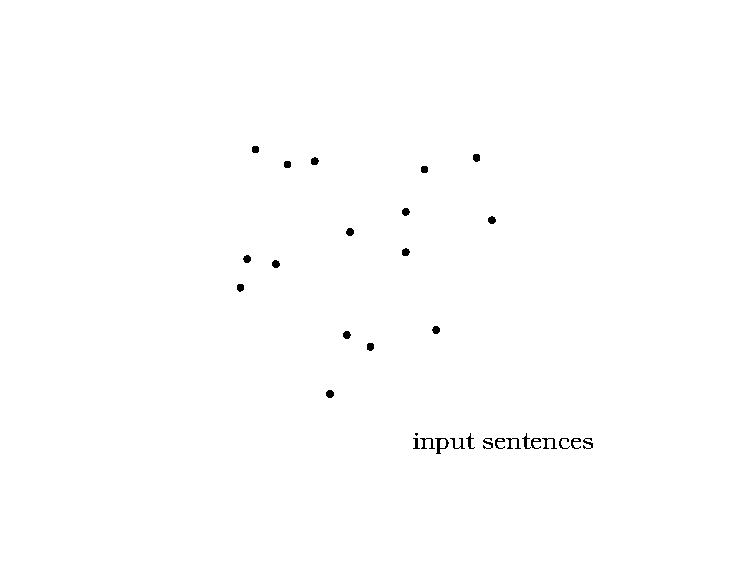
\includegraphics{images/cluster_anim1.pdf}
\end{frame}
\begin{frame}
\frametitle{Affinity Propagation Clustering}
    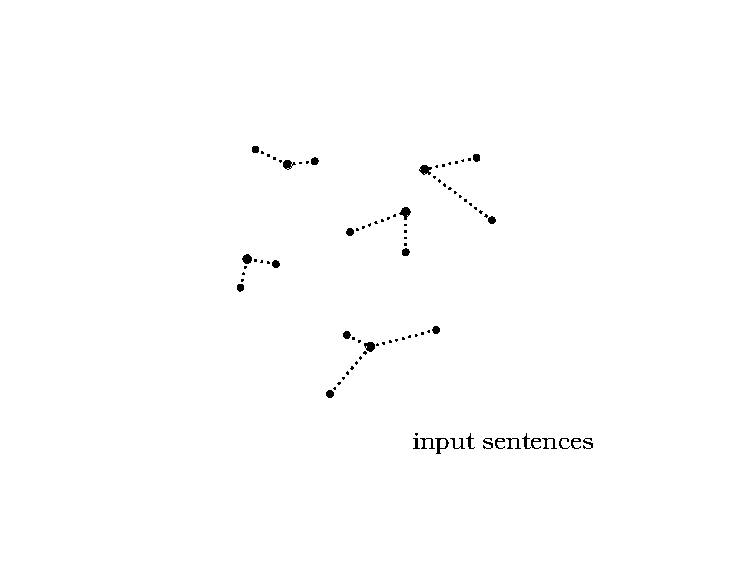
\includegraphics{images/cluster_anim2.pdf}
\end{frame}
\begin{frame}
\frametitle{Affinity Propagation Clustering}
    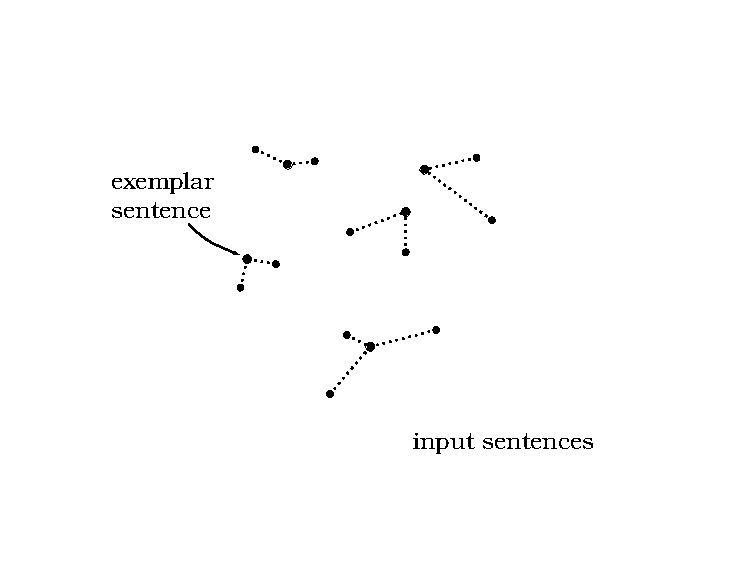
\includegraphics{images/cluster_anim3.pdf}
\end{frame}
\begin{frame}
\frametitle{Affinity Propagation Clustering}
    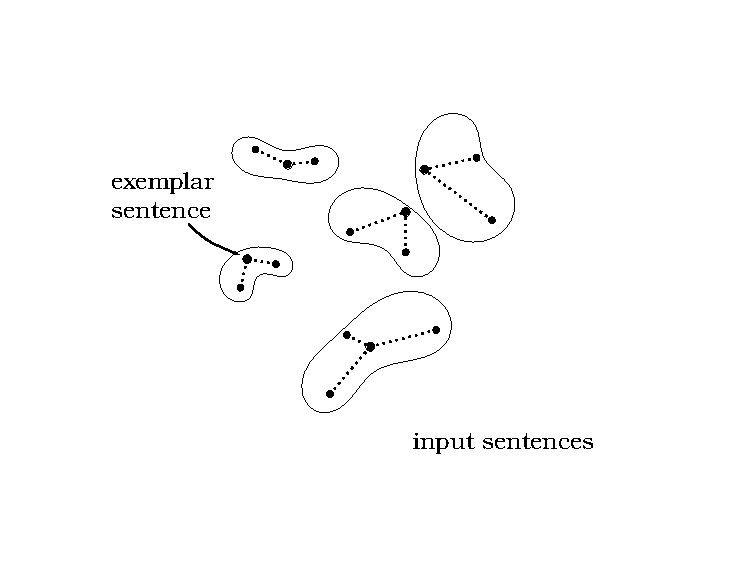
\includegraphics{images/cluster_anim4.pdf}
\end{frame}
\begin{frame}
\frametitle{Affinity Propagation Clustering}
    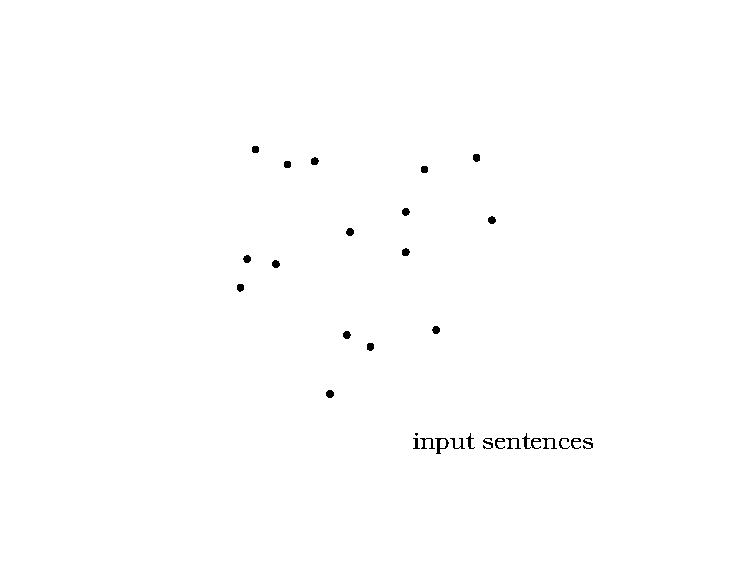
\includegraphics{images/cluster_anim5.pdf}
\end{frame}
\begin{frame}
\frametitle{Affinity Propagation Clustering}
    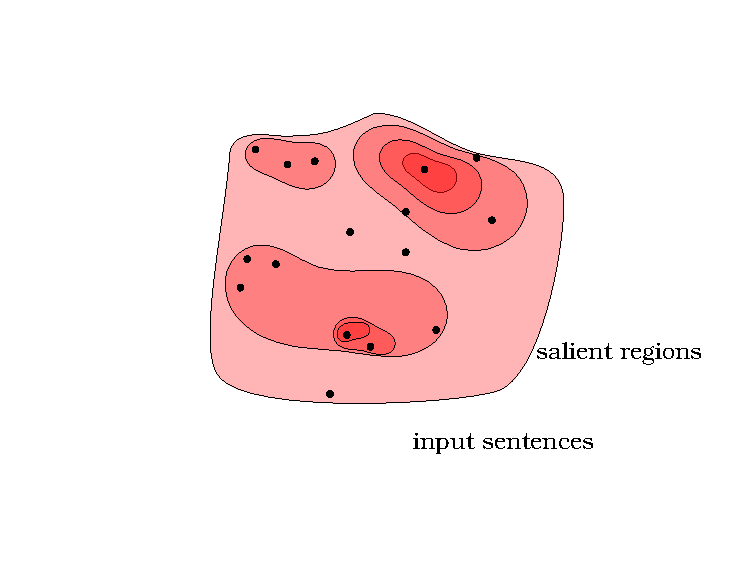
\includegraphics{images/cluster_anim6.pdf}
\end{frame}
\begin{frame}
\frametitle{Affinity Propagation Clustering}
    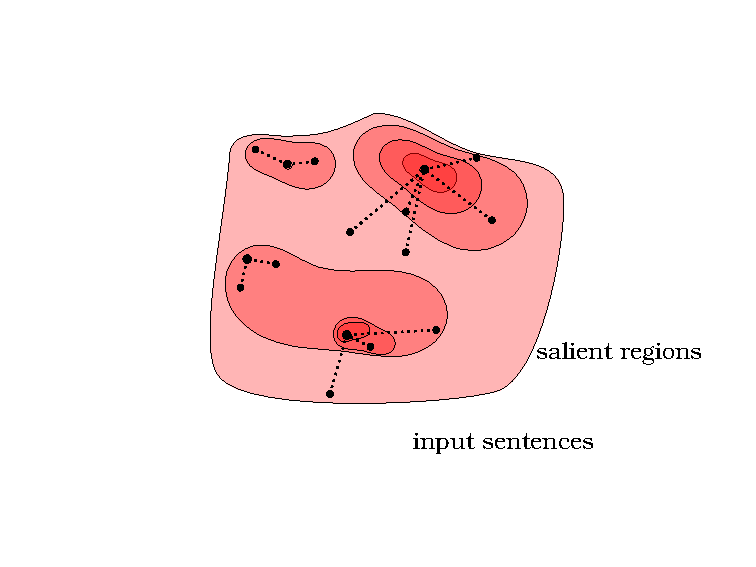
\includegraphics{images/cluster_anim7.pdf}
\end{frame}



%
%
%\begin{frame}
%\frametitle{Information During Disaster}
%\begin{itemize}
%\item \light{People turn to the web and mobile services}
%\item[]
%\item \light{Realtime curation of data requires significant manpower!}
%\begin{itemize}
%\item \textbf{summarizing official information/resources}
%\item \light{summarizing eye witness information}
%\item \light{correcting/updating erroneous information}
%\item \light{predicting likely outcomes}
%\end{itemize}
%\end{itemize}
%\end{frame}
%
%
%\begin{frame}
%\frametitle{Update Summarization}
%\textbf{Given an event:} \pause ``guatemala earthquake''
%\begin{itemize}
%    \item{Monitor a stream of news}
%    \item{Identify relevant information}
%    \item{Update the user}
%        
%\end{itemize}
%    \pause
%    \textbf{CAVEAT:} Updates should be timely and novel! 
%\end{frame}
%
%
%\begin{frame}
%    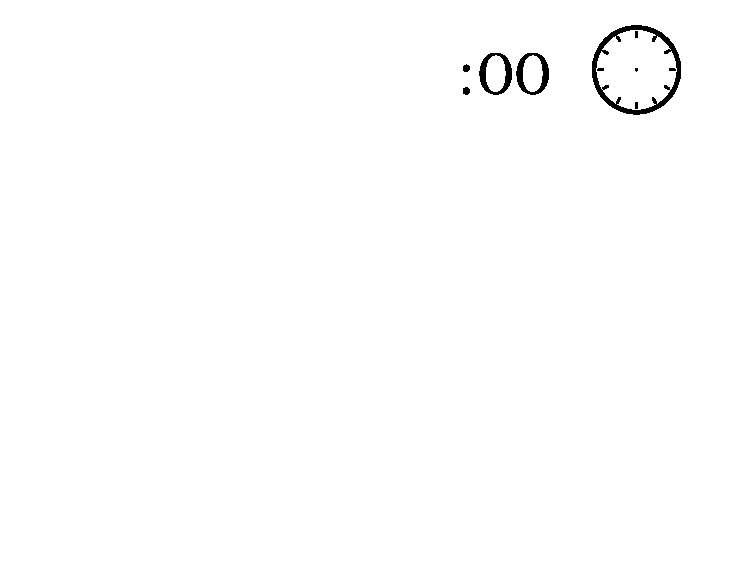
\includegraphics{images/anim1.pdf}
%\end{frame}
%\begin{frame}
%    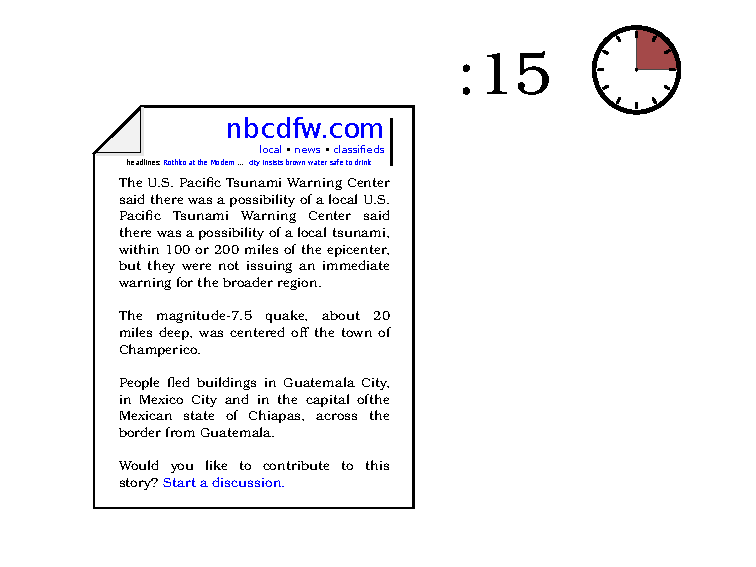
\includegraphics{images/anim2.pdf}
%\end{frame}
%\begin{frame}
%    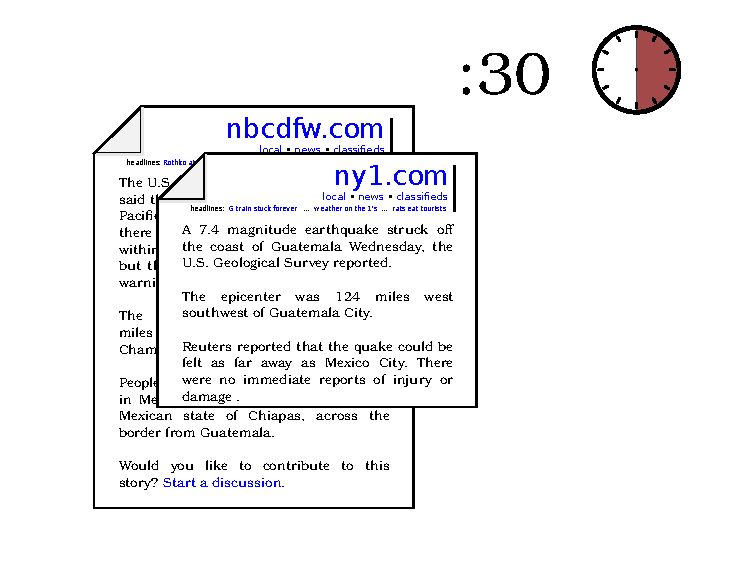
\includegraphics{images/anim3.pdf}
%\end{frame}
%\begin{frame}
%    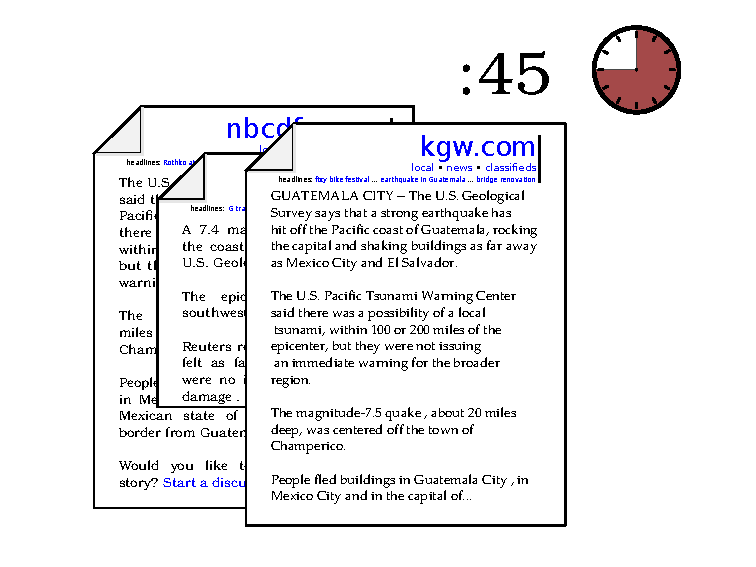
\includegraphics{images/anim4.pdf}
%\end{frame}
%\begin{frame}
%    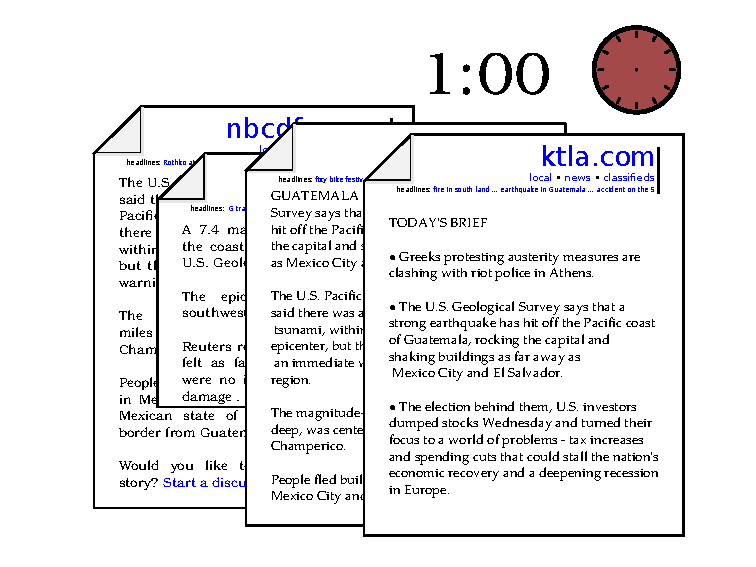
\includegraphics{images/anim5.pdf}
%\end{frame}
%\begin{frame}
%    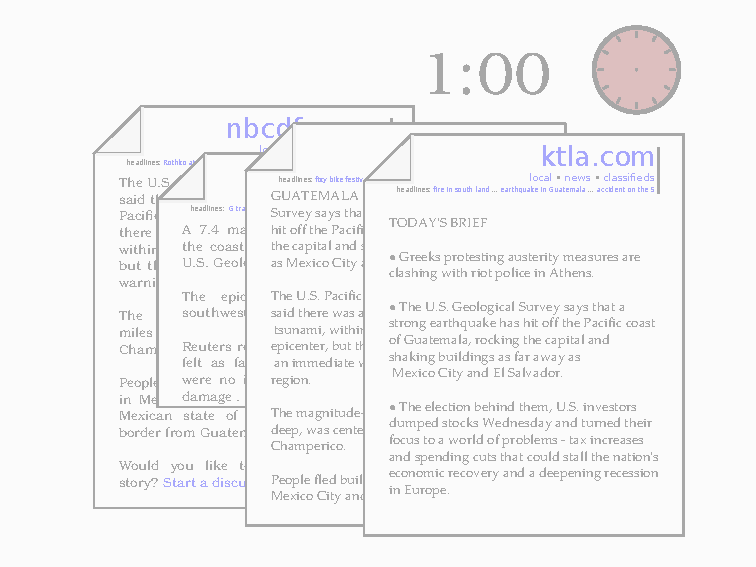
\includegraphics{images/anim6.pdf}
%\end{frame}
%\begin{frame}
%    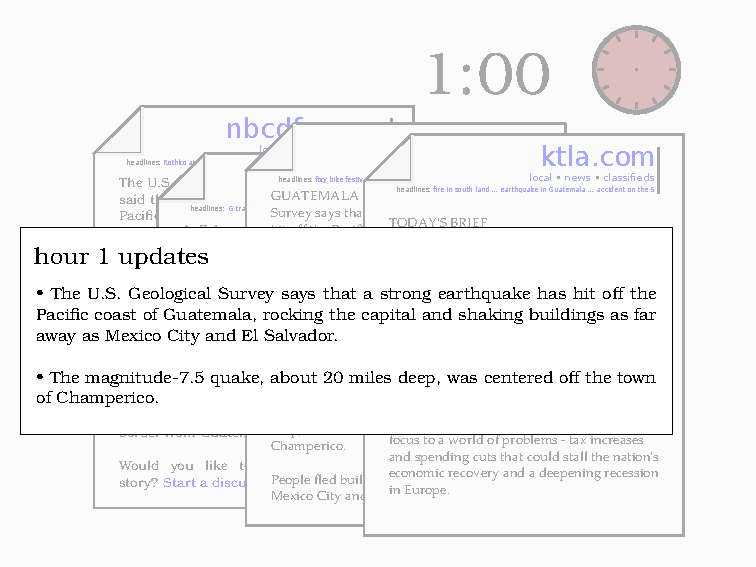
\includegraphics{images/anim7.pdf}
%\end{frame}
%\begin{frame}
%    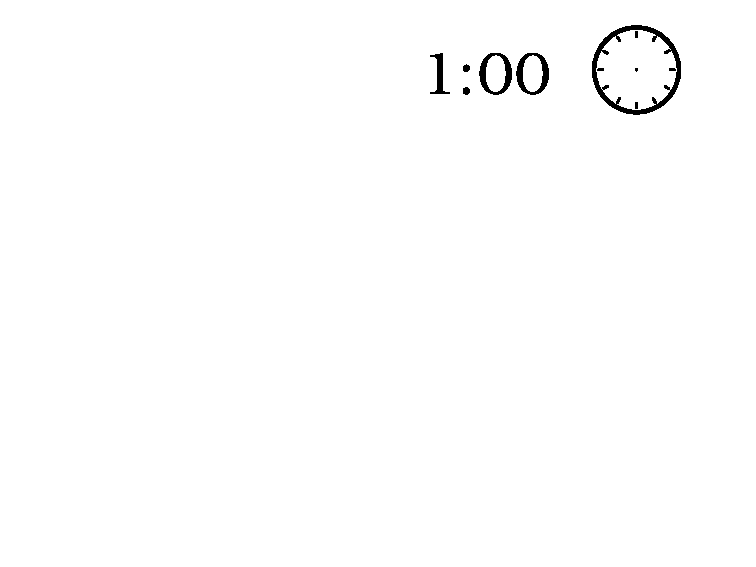
\includegraphics{images/anim8.pdf}
%\end{frame}
%\begin{frame}
%    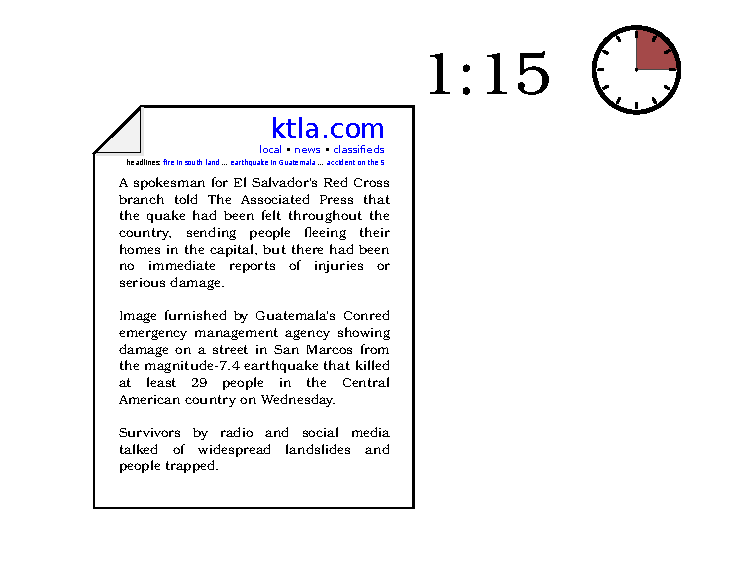
\includegraphics{images/anim9.pdf}
%\end{frame}
%\begin{frame}
%    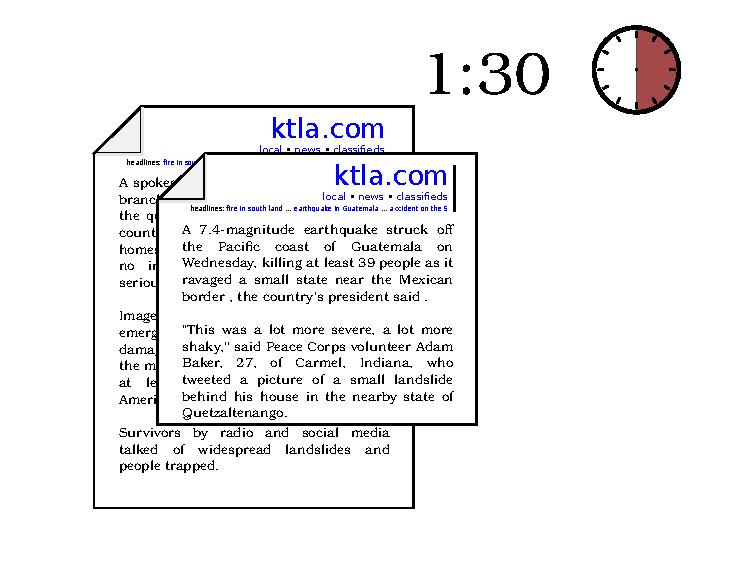
\includegraphics{images/anim10.pdf}
%\end{frame}
%\begin{frame}
%    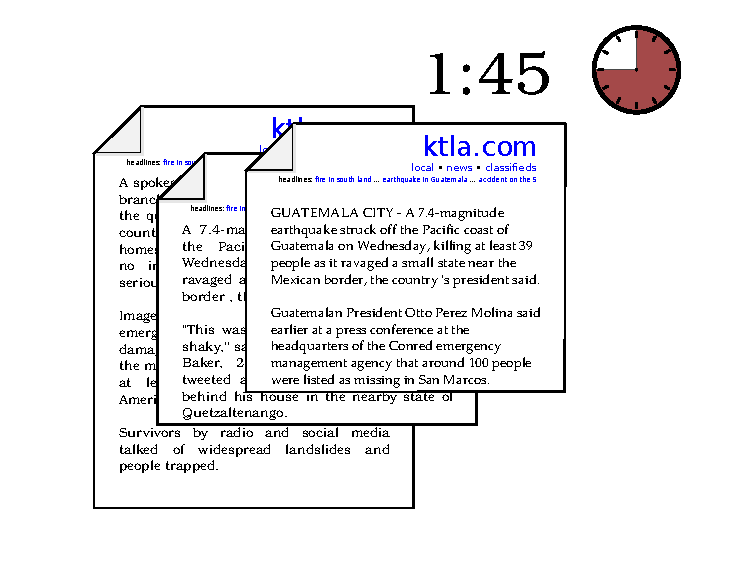
\includegraphics{images/anim11.pdf}
%\end{frame}
%\begin{frame}
%    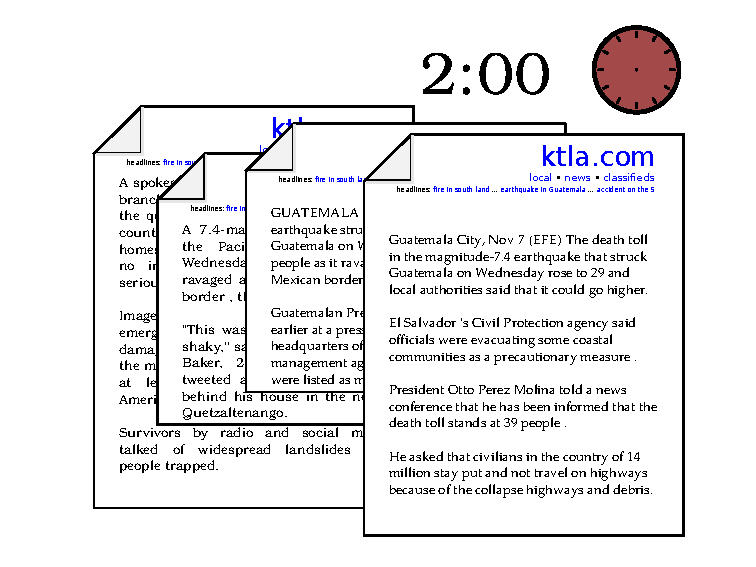
\includegraphics{images/anim12.pdf}
%\end{frame}
%\begin{frame}
%    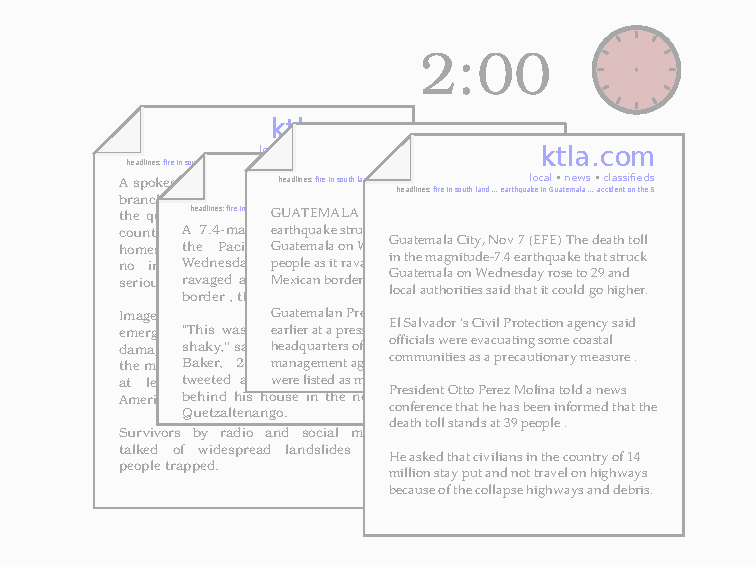
\includegraphics{images/anim13.pdf}
%\end{frame}
%\begin{frame}
%    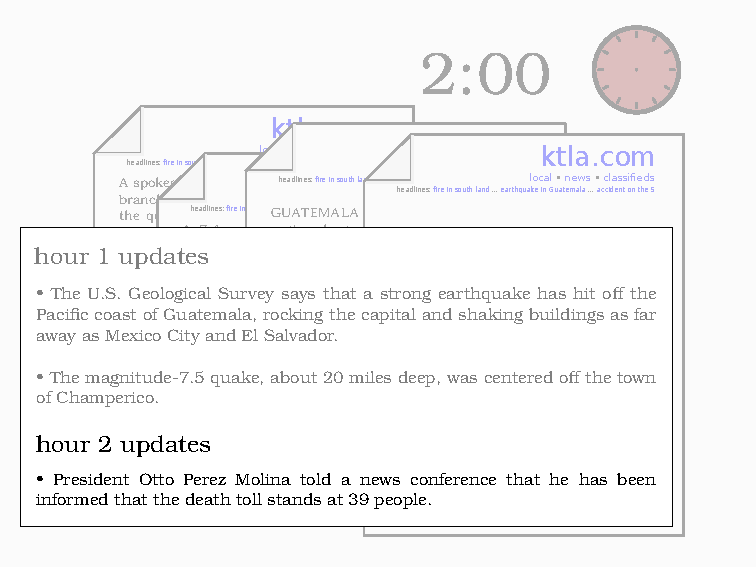
\includegraphics{images/anim14.pdf}
%\end{frame}
%
%\section{Model}
%
%\frame{\tableofcontents[currentsection]}
%\begin{frame}
%\frametitle{Characteristics of a good summary of disaster}
%
%$\pmb{+}$ \textbf{Salience} \\
%Updates should contain the most important information.\\
%~\\
%
%$\pmb{-}$ \textbf{Redundancy} \\
%Updates should focus on new or updated information
%that has not yet been presented to the user.\\
%~\\
%
%$\pmb{-}$ \textbf{Latency} \\
%New information should be delivered as quickly as possible.
%~\\
%
%\end{frame}
%
%
%\begin{frame}
%\frametitle{Update Summarization Approach}
%~\\
%At time $t$:
%\begin{enumerate}
%\item Predict salience for input sentences. 
%\pause
%\begin{itemize}
%\item Domain-specific features for predicting salience
%\end{itemize}
%\pause
%\item Select exemplar sentences for $t$ that are both representative and
%    salient.
%\pause
%%\begin{itemize}
%%\item Incorporate salience predictions in this decision
%%\end{itemize}
%\item Remove redundant sentences.
%%\pause
%\end{enumerate}
%\end{frame}
%
%\subsection{Salience}
%\frame{\tableofcontents[currentsection,currentsubsection]}
%\begin{frame}
%    \frametitle{How do we measure salience?}
%
%    \pause
%
%    event: 2012 Guatemala Earthquake
%    \tikzmark{nuggets}{
%    \begin{itemize}
%        \pause
%        \item epicenter was located in the Pacific Ocean
%        \pause
%    \item \alert<8>{tsunami warnings 100-200 miles from epicenter}
%        \pause
%        \item felt in El Salvador and parts of Mexico
%        \item[] $\;\;\;\;\;\;\;\;\;\vdots \;\;\;\;\;\;\;\;\;\;\;\;\;\;\vdots\;\;\;\;\;\;\;\;\;\;\;\;\;\;\;\vdots$
%        
%    \end{itemize}
%    }
%    \pause
%    \tikz[overlay,remember picture]{
%        \draw[draw=red,thick,double,fill opacity=0.2] ($(nuggets)+(-5.6,-0.2)$) rectangle ($(nuggets)+(2.8,-2.7)$);
%        \node[draw=red,thick,double,fill=white] at ($(nuggets)+(1.7,-2.7)$) {nuggets}; 
%    }
%
%\uncover<7->{\vspace{16pt}
%\pause
%\textit{Nicaragua's disaster management said it had issued a 
%\alert<8>{local tsunami alert.}}\\
%\uncover<9->{
%~\\
%Given a sentence $s$ and a set of gold nuggets $N$, we define the salience 
%of a sentence as
%$$\operatorname{salience}(s) = \max_{n \in N} \operatorname{sim}(s,n).$$
%    }
%}
%\end{frame}
%
%\begin{frame}
%    \frametitle{How do we measure salience?}
%
%    Given a sentence $s$ and a set of gold nuggets $N$, we define the salience 
%    of a sentence as
%    $$\operatorname{salience}(s) = \max_{n \in N} \operatorname{sim}(s,n).$$
%
%    \pause
%    ~\\
%
%    \textbf{Sentence Similarity}\\
%    We use the sentence similarity model of \textit{Guo and Diab, (2012)}\\
%    \begin{itemize}
%        \item model is trained on domain related Wikipedia abstracts
%        \item reduces sentences to a low $k$-dimensional latent vector ($k=100$
%            in our experiments)
%        \item similarity of two sentences is the cosine similarity of their 
%            latent vectors
%    \end{itemize}
%\end{frame}
%
%\begin{frame}
%    \frametitle{How do we measure salience?}
%
%    Given a sentence $s \in S$ and a set of gold nuggets $N$, we define the 
%    salience of a sentence as
%    $$\operatorname{salience}(s) = \max_{n \in N} \operatorname{sim}(s,n).$$
%
%    ~\\
%    $$\uncover<2->{s_1 }\uncover<6->{,\;\; s_2} 
%         \uncover<9->{,\;\; s_3} 
%         \uncover<12->{,\;\; \ldots,\;\; s_k}\uncover<2->{ \sim S}$$
%    ~\\
%    \begin{center}
%    \uncover<3->{
%    \begin{tabular}{c | c }
%        $y$ & $X$\\[2pt]
%    \hline
%    \uncover<4->{$\operatorname{salience}(s_1)$} & \uncover<5->{\alert<17>{$\phi(s_1)$}}\\[2pt]
%    \uncover<7->{$\operatorname{salience}(s_2)$} & \uncover<8->{\alert<17>{$\phi(s_2)$}}\\[2pt] 
%    \uncover<10->{$\operatorname{salience}(s_3)$} & \uncover<11->{\alert<17>{$\phi(s_3)$}}\\[2pt]
%    \uncover<13->{$\vdots$} & \uncover<14->{$\vdots$}\\[2pt]    
%    \uncover<15->{$\operatorname{salience}(s_k)$} & \uncover<16->{\alert<17>{$\phi(s_k)$}}\\[2pt]
%    \end{tabular}
%    }
%    \end{center}
%\end{frame}
%\subsection{Model Features}
%\frame{\tableofcontents[currentsection,currentsubsection]}
%\begin{frame}
%\frametitle{Predicting Salience: Model Features}
%\begin{itemize}
%\item Basic sentence level features
%\begin{itemize}
%\item sentence length
%\item punctuation count
%\item \alert<2-4>{number of capitalized words}
%\item sentence position in document
%\end{itemize}
%\end{itemize}
%
%\pause
%\textbf{High Salience}\\ 
%\alert<2>{Nicaragua's} disaster management said it had issued a local tsunami alert.\\
%\textbf{Medium Salience} \\
%\alert<3>{People} streamed out of homes, schools and office buildings as far north as \alert<3>{Mexico City.}\\
%
%\textbf{Low Salience} \\
%\alert<4>{Add} to \alert<4>{Digg Add} to del.icio.us \alert<4>{Add} to \alert<4>{Facebook Add} to \alert<4>{Myspace} 
%
%\end{frame}
%
%\begin{frame}
%\frametitle{Predicting Salience: Model Features}
%\begin{itemize}
%\item Basic sentence level features
%\item Query features
%\begin{itemize}
%\item query term matches
%\item event type synonym, \alert<2>{hypernym}, and hyponym matches
%\end{itemize}
%\end{itemize}
%
%\textbf{High Salience}\\ 
%Nicaragua's \alert<2>{disaster} management said it had issued a local tsunami alert.\\
%\textbf{Medium Salience} \\
%People streamed out of homes, schools and office buildings as far north as 
%Mexico City.\\
%
%\textbf{Low Salience} \\
%Add to Digg Add to del.icio.us Add to Facebook Add to Myspace
%
%\end{frame}
%
%
%\begin{frame}
%\frametitle{Predicting Salience: Model Features}
%\begin{itemize}
%\item Basic sentence level features
%\item Query features
%\item Language Models (5-gram interpolated Kneser-Ney model)
%\begin{itemize}
%\item \alert<2>{generic news corpus (10 years of AP and NY Times articles)}
%\item \alert<4>{domain specific corpus (domain related Wikipedia articles)}
%\end{itemize}
%\end{itemize}
%
%\pause
%\textbf{High Salience}\\ 
%\alert<2,4>{Nicaragua's disaster management said it had issued a local tsunami alert.}\\
%\textbf{Medium Salience} \\
%\alert<2>{People streamed out of homes, schools and office buildings as far north as Mexico City.}\\
%\textbf{Low Salience} \\
%Add to Digg Add to del.icio.us Add to Facebook Add to Myspace 
%
%
%\end{frame}
%
%
%\begin{frame}
%\frametitle{Predicting Salience: Model Features}
%\begin{itemize}
%\item Basic sentence level features
%\item Query features
%\item Language Models
%\item Geographic Features
%\begin{itemize}
%\item input sentences tagged with Named-Entity tagger
%\item coordinates are retrieved for each location in a sentence
%\item mean distance to event
%\end{itemize}
%\end{itemize}
%
%\pause
%\textbf{High Salience}\\ 
%\alert<2>{Nicaragua's} disaster management said it had issued a local tsunami alert.\\
%\textbf{Medium Salience} \\
%People streamed out of homes, schools and office buildings as far north as \alert<2>{Mexico City.}\\
%\textbf{Low Salience} \\
%Add to Digg Add to del.icio.us Add to Facebook Add to Myspace 
%
%
%
%\end{frame}
%
%\begin{frame}
%\frametitle{Predicting Salience: Model Features}
%\begin{itemize}
%\item Basic sentence level features
%\item Query features
%\item Language Models (5-gram interpolated Kneser-Ney model)
%\item Geographic Features
%\item Temporal Features
%\begin{itemize}
%\item average tf-idf at the current time $t_0$
%\item difference of average tf-idf at time $t_0$ and $t_{-1}$
%\item $\;\;\;\;\;\;\;\;\;\vdots$
%\item difference of average tf-idf at time $t_0$ and $t_{-24}$
%\item hours since event start time
%\end{itemize}
%\end{itemize}
%
%
%\pause
%\textbf{High Salience}\\ 
%\alert<2>{Nicaragua's disaster management} said it had issued a local \alert<2>{tsunami} alert.\\
%\textbf{Medium Salience} \\
%People streamed out of homes, schools and office buildings as far north as Mexico City.\\
%\textbf{Low Salience} \\
%\alert<3>{Add to Digg Add to del.icio.us Add to Facebook Add to Myspace} 
%
%\end{frame}
%
%\subsection{Update Selection}
%\frame{\tableofcontents[currentsection,currentsubsection]}
%\begin{frame}
%\frametitle{Affinity Propagation Clustering}
%\begin{itemize}
%\pause
%\item assigns each data point to an exemplar data point \\
%     (these assignments
%      define a cluster)
%\pause
%\item exemplars are actual data points that best represent their cluster
%\pause
%\item exemplar selection is determined by a similarity matrix $S$ and 
%      exemplar \textit{preference}
%\pause
%\begin{itemize}
%\pause 
%\item similarities $S$ -- element $s(i,j)$ is the semantic similarity of sentence $i$ to sentence $j$
%\pause
%\item \textit{preference} -- scalar value that represents 
%      apriori how suited a data point is to be an exemplar
%\pause
%\item \alert<+->{preference $=$ salience}
%\pause
%\item \alert<+->{exemplar $=$ update}
%\end{itemize}
%
%\end{itemize}
%%\begin{columns}[T]
%%\column{0.5\textwidth}
%%$$r(i,k) \leftarrow s(i,k) - \max_{k^\prime\ne k} a(i,k^\prime) 
%%+ s(i,k^\prime) $$
%
%%\column{0.5\textwidth}
%%    Update 2
%%\end{columns}
%
%\end{frame}
%
%
%
%
%\section{Data}
%\frame{\tableofcontents[currentsection,currentsubsection]}
%
%\begin{frame}
%\frametitle{Trec Temporal Summarization Track}
%\begin{itemize}
%\pause
%\item TREC KBA Stream Corpus
%\pause
%\begin{itemize}
%\item hourly web crawl
%\item October 2011 - February 2013
%\item 16.1TB!
%\end{itemize}
%\pause
%\item[]
%\item Training Data
%\begin{itemize}
%\item Training Events
%\end{itemize}
%\end{itemize}
%\end{frame}
%
%\begin{frame}
%\frametitle{Trec TS Events}
%\begin{itemize}
%    \item{Natural Disasters}
%        \begin{itemize}
%            \item{\textbf{2012 Guatemalan Earthquake}}
%            \item{Hurricane Sandy\\}
%            $\;\;\;\;\;\;\;\;\vdots$
%        \end{itemize}
%    \item{Man-made Disasters}
%        \begin{itemize}
%            \item{2012 Pakistan Garment Factory Fires}
%            \item{2012 Buenos Aires Rail Disaster\\}
%            $\;\;\;\;\;\;\;\;\vdots$
%        \end{itemize}
%    \item{Terrorism/Violence}
%    \item{Social Unrest}
%\end{itemize}
%\end{frame}
%%\begin{frame}
%%put pic of doc frequency over time
%
%\begin{frame}
%\frametitle{Trec Temporal Summarization Track}
%\begin{itemize}
%\item TREC KBA Stream Corpus
%\begin{itemize}
%\item hourly web crawl
%\item October 2011 - February 2013
%\item 16.1TB!
%\end{itemize}
%\item[]
%\item Training Data
%\begin{itemize}
%\item Training Events
%\pause
%\item Gold Nugget Information
%\end{itemize}
%\end{itemize}
%\end{frame}
%
%
%\begin{frame}
%\frametitle{Gold Nugget Information}
%\begin{itemize}
%\item epicenter was located in the Pacific Ocean 
%%\item[]
%\item tsunami warnings 100-200 miles from epicenter
%%\item[]
%\item felt in El Salvador and parts of Mexico
%\end{itemize}
%\end{frame}
%
%\begin{frame}
%\frametitle{Extracting Gold Nuggets from Wikipedia}
%%SYSTEM TIME: 2012-11-07-19\\
%\vspace{5pt}
%\includegraphics[width=325pt,height=200pt]{png/wp_evo_1}
%\end{frame}
%\begin{frame}
%\frametitle{Extracting Gold Nuggets from Wikipedia}
%%SYSTEM TIME: 2012-11-07-20\\
%\vspace{5pt}
%\includegraphics[width=325pt,height=200pt]{png/wp_evo_2}
%\end{frame}
%\begin{frame}
%\frametitle{Extracting Gold Nuggets from Wikipedia}
%%SYSTEM TIME: 2012-11-08-05\\
%\vspace{5pt}
%\includegraphics[width=325pt,height=200pt]{png/wp_evo_3}
%\end{frame}
%\begin{frame}
%\frametitle{Extracting Gold Nuggets from Wikipedia}
%%SYSTEM TIME: 2012-11-08-05\\
%\vspace{5pt}
%\includegraphics[width=325pt,height=200pt]{png/wp_evo_4}
%\end{frame}
%
%\begin{frame}
%\frametitle{Extracting Gold Nuggets from Wikipedia}
%%SYSTEM TIME: 2012-11-08-05\\
%\vspace{5pt}
%\includegraphics[width=325pt,height=200pt]{png/wp_evo_3}
%\end{frame}
%
%\begin{frame}
%\frametitle{Extracting Gold Nuggets from Wikipedia}
%%SYSTEM TIME: 2012-11-08-05\\
%\vspace{5pt}
%\includegraphics[width=325pt,height=200pt]{png/wp_evo_5}
%\end{frame}
%
%\begin{frame}
%\frametitle{Trec Temporal Summarization Track}
%\begin{itemize}
%\item TREC KBA Stream Corpus
%\begin{itemize}
%\item hourly web crawl
%\item October 2011 - February 2013
%\item 16.1TB!
%\end{itemize}
%\item[]
%\item Training Data
%\begin{itemize}
%\item Training Events
%\item Gold Nugget Information
%\end{itemize}
%\end{itemize}
%\end{frame}
%
%
%
%\section{Experiments}
%\frame{\tableofcontents[currentsection,currentsubsection]}
%
%\begin{frame}
%    \frametitle{Experiments}
%    
%    \begin{itemize}
%        \pause
%        \item leave one out evaluation on 21 TREC TS events
%        \pause
%        \item 3 events held out for tuning similarity threshold parameters
%        \pause
%        \item trained salience models for each event
%        \pause
%        \begin{itemize}
%            \item 1000 sentences sampled for each event
%            \item at test time, salience prediction is the average of the 
%                23 other models
%        \end{itemize}
%    \end{itemize}
%    
%\end{frame}
%
%\begin{frame}
%    \frametitle{Evaluation Metrics}
%    \begin{itemize}
%        \pause
%        \item ROUGE 
%        \pause
%        \begin{itemize}
%            \item model summary generated by concatenating event nuggets
%        \end{itemize}
%        \pause
%    \item Expected Gain and Comprehensiveness
%        $$\mathbb{E}[\mathrm{Gain}] = \frac{|S_n|}{|S|}\;\;\;\;\;\;\;\;\;
%            \textrm{Comprehensiveness} = \frac{|S_n|}{|N|}$$
%            where \begin{itemize}
%                    \pause
%            \item[] $S$ is the set of system updates
%                    \pause
%                \item[] $S_n$ is the set of nuggets mapped to updates in $S$
%                    \pause
%                \item[] $N$ is the set of nuggets for the event
%            \end{itemize}
%    \end{itemize}
%\end{frame}
%
%\begin{frame}
%    \frametitle{Baselines}
%    \begin{itemize}
%    \item AP+Salience -- full model
%    \item AP -- affinity propagation clustering with no salience
%    \item HAC -- hierarchical agglomerative clustering
%    \item RS -- rank by salience
%    \end{itemize}
%\end{frame}
%
%\begin{frame}
%    \frametitle{ROUGE}
%\begin{table}[h]
%\centering
%% centering table
%\begin{tabular}{l c c c}
%% creating 10 columns
%\multicolumn{4}{c}{ROUGE-1}\\
%\hline
%\hline
%% inserting double-line
%$\mathrm{System}$ & $\mathrm{Recall}$ & $\mathrm{Prec.}$ & $\mathrm{F}_1$\\
%[0.5ex]
%\hline
%AP+Salience & $\mathbf{0.282}$ & $\mathbf{0.344}$ & $\mathbf{0.306}$\\
%AP          & $0.245$ & $0.285$ & $0.263$ \\
%RS          & $0.230$ & $0.271$ & $0.247$ \\
%HAC         & $0.169$ & $0.230$ & $0.186$ \\
%\hline % inserts single-line
%\end{tabular}
%~\\[1ex]
%~\\
%\begin{tabular}{l c c c}
%% creating 10 columns
%\multicolumn{4}{c}{ROUGE-2}\\
%\hline
%\hline
%% inserting double-line
%$\mathrm{System}$ & $\mathrm{Recall}$ & $\mathrm{Prec.}$ & $\mathrm{F}_1$\\[0.5ex]
%\hline
%\textsc{AP+Salience} & $\mathbf{0.045}$ & $\mathbf{0.056}$ & $\mathbf{0.049}$\\
%\textsc{AP}          & $0.033$ & $0.038$ & $0.035$ \\
%\textsc{RS}          & $0.031$ & $0.037$ & $0.034$ \\
%\textsc{HAC}         & $0.017$ & $0.024$ & $0.019$ \\
%\hline % inserts single-line
%\end{tabular}
%\end{table}
%\end{frame}
%
%
%\begin{frame}
%\frametitle{ROUGE-1 over time}
%\begin{center}
%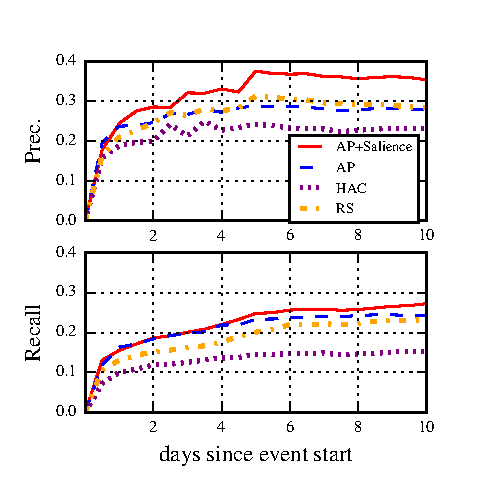
\includegraphics[]{images/rouge-time.eps}
%\end{center}
%\end{frame}
%
%
%\begin{frame}
%\frametitle{$\mathbb{E}[\mathrm{Gain}]$ and $\mathrm{Comprehensiveness}$}
%\begin{center}
%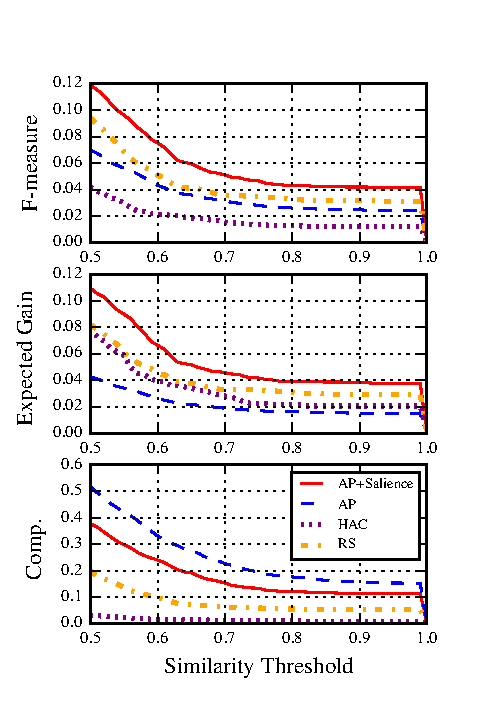
\includegraphics[scale=.7]{images/nuggets-metrics2.eps}
%\end{center}
%\end{frame}
%
%\section{Conclusion}
%\begin{frame}
%\frametitle{Future Work}
%
%\begin{itemize}
%\item Online update summarization
%\pause
%\item[]
%\item Improved redundancy
%\end{itemize}
%\end{frame}
%
%\begin{frame}
%\frametitle{Links}
%
%\begin{itemize}
%\item Trec Temporal Summarization Track \\ 
%    \begin{center}\url{http://www.trec-ts.org}\end{center}
%\item[]
%\item ACL paper\\\begin{center} \url{http://www.columbia.edu/~crk2130}\end{center}
%\end{itemize}
%
%\end{frame}
%
\end{document}
